% coding:utf-8

% Ausführen in R: 
% Sweave("C:/Daten/Daniel/studium/git_repo/sem2/stoc/sw10/sw10_2.Rnw",encoding='UTF-8')

\section{Aufgabe 2}

\subsection{a}
Es handelt sich um ungepaarte Stichproben. 

\subsection{b}

\subsection{c}
\begin{Schunk}
\begin{Sinput}
> # jackals=read.table("http://stat.ethz.ch/Teaching/Datasets/jackals.dat", header=TRUE)
> jackals=read.table("jackals.dat", header=TRUE)
> t.test(jackals[,'M'], jackals[,'W'], var.equal = TRUE)
\end{Sinput}
\begin{Soutput}
	Two Sample t-test

data:  jackals[, "M"] and jackals[, "W"] 
t = 3.4843, df = 18, p-value = 0.002647
alternative hypothesis: true difference in means is not equal to 0 
95 percent confidence interval:
 1.905773 7.694227 
sample estimates:
mean of x mean of y 
    113.4     108.6 
\end{Soutput}
\end{Schunk}

\subsection{d}
\begin{Schunk}
\begin{Sinput}
> wilcox.test(jackals[,'M'], jackals[,'W'], var.equal = TRUE)
\end{Sinput}
\begin{Soutput}
	Wilcoxon rank sum test with continuity correction

data:  jackals[, "M"] and jackals[, "W"] 
W = 87.5, p-value = 0.004845
alternative hypothesis: true location shift is not equal to 0 
\end{Soutput}
\end{Schunk}

\subsection{e}
\begin{Schunk}
\begin{Sinput}
> qqnorm(jackals[,"M"])
> qqline(jackals[,"M"],col='green')
\end{Sinput}
\end{Schunk}
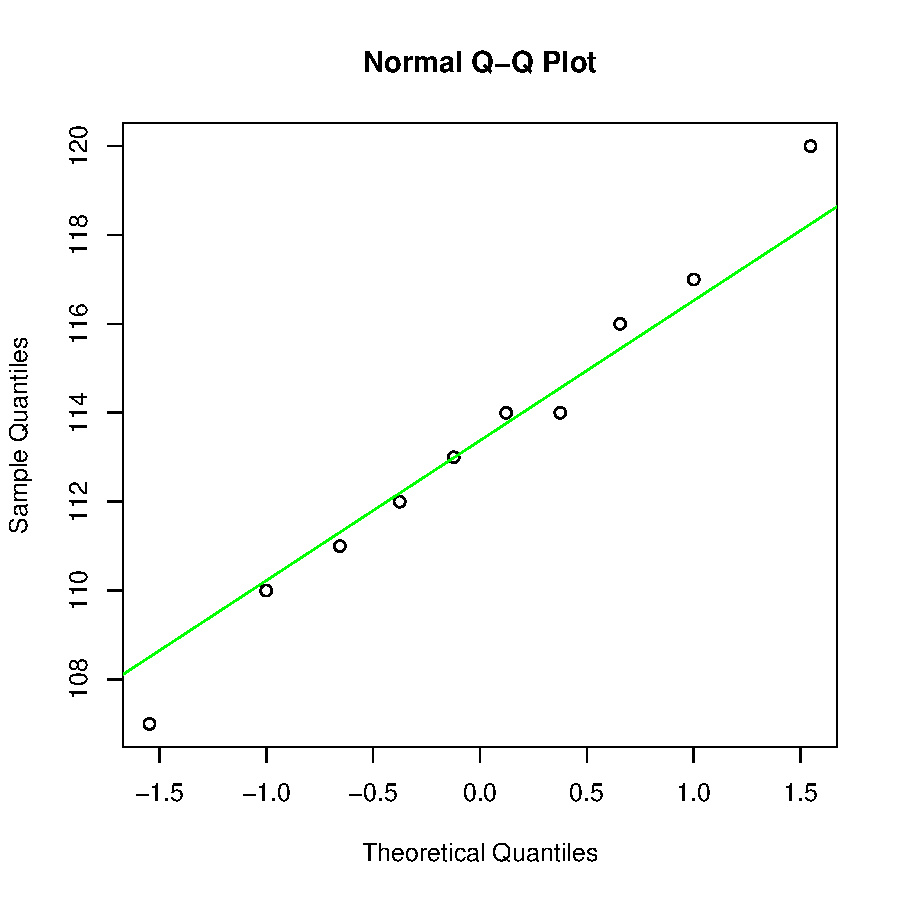
\includegraphics{sw11_2-003}
\begin{Schunk}
\begin{Sinput}
> qqnorm(jackals[,"W"])
> qqline(jackals[,"W"],col='green')
\end{Sinput}
\end{Schunk}
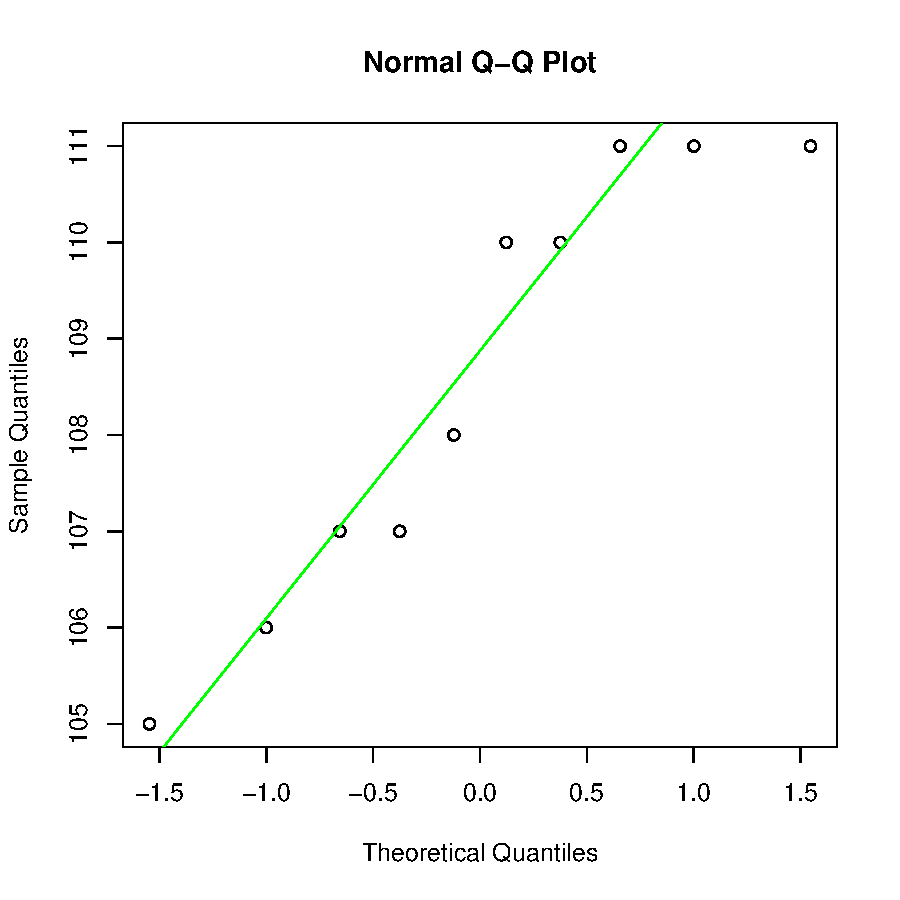
\includegraphics{sw11_2-004}
